Accurate detection of specific oligonucleotide sequences is of crucial importance in biomedical research and in the early diagnosis disorders whose action is regulated by microRNA/DNA, such as cancer, but also viral, immune-related, and neurodegenerative diseases \parencite{li_micrornas_2012}.
Peptide Nucleic Acids (PNAs) are nucleic acid mimics, whose properties make it an interesting candidate for probing micro-RNA/DNA presence. Most notably, neutrality of the backbone confers great selectivity to target sequences and stability of duplexes.
Current applications of PNA in nucleic acid sensing focuses on  rely on labeling or chemical reactions \parencite{saarbach2019peptide}, which can may require careful managing of reactants concentration for correct usage.

On the other hand, we will discuss a label-free setup that does not involve chemical processes, thus being potentially simpler and more robust, while ensuring high selectivity and sensitivity to target sequences.
A schematic representation of the system is shown in Fig.\ref{schematic_system}: PNA is linked at one end to the diamond substrate and is in solution with water, Cl$^-$ and Mn$^{2+}$ ions.
\begin{figure}[h]
    \centering
    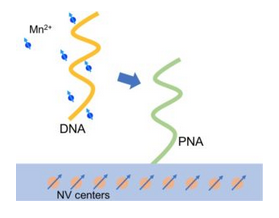
\includegraphics[width=0.5\linewidth]{schematic_system_.png}
    \caption{Schematic representation of the system. PNA is in solution and linked to the diamond substrate. Since DNA/RNA is negatively charged, it coordinates Mn$^{2+}$ ions that are brought close to the surface upon hybridisation. }
    \label{schematic_system}
\end{figure}

The main idea is that, if target RNA/DNA sequences are present in solution, upon duplex formation, Mn$^{2+}$ ions will coordinate around the double helix, resulting in the accumulation of cations in the proximity of the substrate.
This setup exploits the sensitivity of fluorescence by Nitrogen-Vacancy centers to the local concentrations of paramagnetic species, such as Mn$^{2+}$, which is how  the presence of target nucleic acid (NA) sequences can ultimately be revealed.

In particular, this work addresses the computational modeling of this system, through molecular dynamics simulations and subsequent data analysis.

\section{Objectives}

Overall dynamics of the hybrid RNA-PNA structures need to be addressed for helping rational design of the system and interpretation of data.
Moreover, interaction with the functionalised diamond surface may play a fundamental role and lend significant differences in the kinetics and properties of the system. Lastly, we will discuss Mn$^{2+}$ coordination around the duplexes and how it affects their influence on NV-centers fluorescence.

*
Risposta in funzione della concentrazione?
Concentrazione threshold?
*

\section{Nucleic Acid Sensing}

MicroRNAs (miRNAs) are short ($~ 20$ nucleotides) noncoding RNAs moleculs involved in physiological processes such as regulation of post-transcriptional gene expression and RNA silencing in animals, plants and some viruses \parencite{bartel_micrornas_2009}.
Their misregulation has been shown to be implicated in common diseases such as Parkinson's, Alzheimer's, HIV-1, multiple sclerosis, type II diabetes, different forms of cancer, etc (see \parencite{li_micrornas_2012} for a complete review on the role of miRNA on common human diseases).
Probing the presence of such oligonicleotides is a crucial aspect in diagnosis and medical research


\section{Nitrogen-Vacancy Centers}

\section{Peptide Nucleic Acids (PNA)}

